% Copyright (c) 2015 Daniele Masini - d.masini.it@gmail.com

\section{Esercizi}

\subsection{Esercizi riepilogativi}

\begin{esercizio}
\label{ese:2.1}
In base alla figura a lato rispondi alle seguenti domande\\
\begin{minipage}{.7\linewidth}
\begin{enumeratea}
\item Il lato \(AB\) si oppone all'angolo \ldots\ldots\ldots
\item L'angolo \(\alpha\) si oppone al lato \ldots\ldots\ldots
\item L'angolo di vertice \(C\) si chiama \ldots\ldots\ldots
\item L'angolo \(\gamma\) è adiacente ai lati \ldots\ldots{} e 
\ldots\ldots
\item I lati \(AB\) e \(BC\) sono adiacenti all'angolo \ldots\ldots
\item I lati \(AC\) e \(AB\) formano l'angolo \ldots\ldots
\item Traccia l'angolo esterno al triangolo nel vertice \(A\)
\item Traccia la bisettrice dell'angolo \(\beta\)
\item Traccia l'altezza relativa alla base \(AB\)
\item Traccia la mediana relativa al lato \(BC\)
\end{enumeratea}
\end{minipage}\hfil
\begin{minipage}{.3\linewidth}
%\begin{wrapfigure}{r}{0pt}
  \centering
    % Copyright (c) 2015 Daniele Masini - d.masini.it@gmail.com

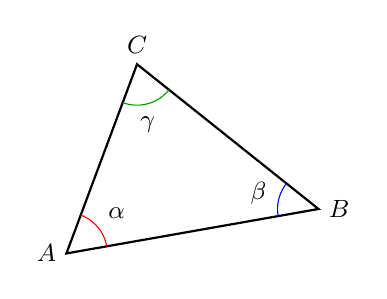
\begin{tikzpicture}[scale=1.3,font=\small]
\usetikzlibrary{calc}

\begin{scope}[rotate=10]
\coordinate (a) at (0,0);
\coordinate (c) at (1,1.7);
\coordinate (b) at (2.5,0);

\draw[thick] (b) node[right] {$B$} -- (c) node[above] {$C$} -- (a) node[left] {$A$} -- cycle;

\begin{scope}
\clip (a) -- (b) -- (c) -- cycle;
\draw[red] (a) circle (0.4);
\node at ([shift={(.55,.3)}]a) {$\alpha$};
\draw[blue] (b) circle (0.4);
\node at ([shift={(-.55,.25)}]b) {$\beta$};
\draw[green!60!black] (c) circle (0.4);
\node at ([shift={(0,-.6)}]c) {$\gamma$};
\end{scope}

\end{scope}

\end{tikzpicture}

%\end{wrapfigure}
\end{minipage}
\end{esercizio}

\begin{esercizio}
\label{ese:2.2}
Disegna un segmento \(AB\), quindi disegna i triangoli \(ABC\) e \(ABD\) 
che hanno la base \(AB\) in comune.
\end{esercizio}

\begin{esercizio}
\label{ese:2.3}
Disegna le tre altezze di ciascuno dei triangoli nella 
figura~\ref{fig:ese2.3}.
\end{esercizio}


\begin{inaccessibleblock}[Figura: TODO]
 \begin{figure}[htb]
\centering% Copyright (c) 2015 Daniele Masini - d.masini.it@gmail.com

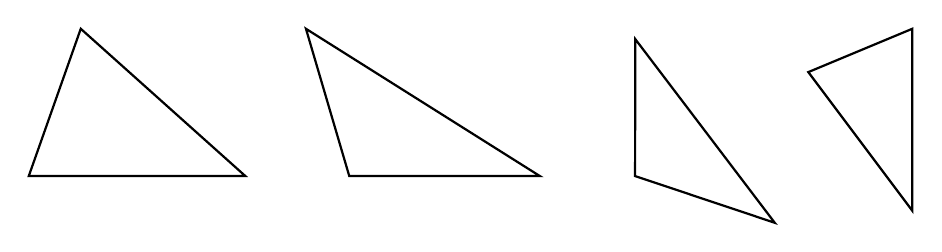
\begin{tikzpicture}[scale=1.1,font=\small]
\usetikzlibrary{calc}

\begin{scope}
\coordinate (a) at (0,0);
\coordinate (c) at (0.6,1.7);
\coordinate (b) at (2.5,0);
\draw[thick] (b)-- (c) -- (a) -- cycle;
\end{scope}

\begin{scope}[xshift=3.7cm]
\coordinate (a) at (0,0);
\coordinate (c) at (-.5,1.7);
\coordinate (b) at (2.2,0);
\draw[thick] (b)-- (c) -- (a) -- cycle;
\end{scope}

\begin{scope}[xshift=7cm, rotate=-18.5]
\coordinate (a) at (0,0);
\coordinate (c) at (-.5,1.5);
\coordinate (b) at (1.7,0);
\draw[thick] (b)-- (c) -- (a) -- cycle;
\end{scope}

\begin{scope}[xshift=9cm]
\coordinate (a) at (0,1.2);
\coordinate (c) at (1.2,1.7);
\coordinate (b) at (1.2,-0.4);
\draw[thick] (b)-- (c) -- (a) -- cycle;
\end{scope}


\end{tikzpicture}

\caption{Esercizio~\ref{ese:2.3}}\label{fig:ese2.3}
\end{figure}
\end{inaccessibleblock}

\begin{esercizio}
\label{ese:2.4}
Per ciascuna delle coppie di triangoli a lato indica se sono 
congruenti ed eventualmente per quale criterio.\\
\begin{minipage}{.5\linewidth}
\begin{enumeratea}
\item Si sa che sono congruenti i lati \(AB\) con \(A'B'\) e \(AC\) con 
\(A'C'\), l'angolo \(\widehat{A}\) con l'angolo \(\widehat{A'}\).\\
I triangoli sono congruenti?\tab	Sì\quad	No\\
Se sì, per il \ldots\ldots\ldots\ldots\ldots\ldots\ldots\ldots

\item Si sa che sono congruenti i lati \(AB\) con \(A'B'\) e gli angoli 
\(\widehat{A}\) con \(\widehat{B'}\) e \(\widehat{B}\) con \(\widehat{A'}\).\\
I triangoli sono congruenti?\tab	Sì\quad	No\\
Se sì, per il \ldots\ldots\ldots\ldots\ldots\ldots\ldots\ldots

\item Si sa che sono congruenti i lati \(AB\) con \(A'B'\) e \(BC\) con 
\(A'C'\), l'angolo \(\widehat{A}\) con \(\widehat{A'}\).\\
I triangoli sono congruenti?\tab	Sì\quad	No\\
Se sì, per il \ldots\ldots\ldots\ldots\ldots\ldots\ldots\ldots
\end{enumeratea}
\end{minipage}\hfil
\begin{minipage}{.4\linewidth}
  \centering
    % Copyright (c) 2015 Daniele Masini - d.masini.it@gmail.com

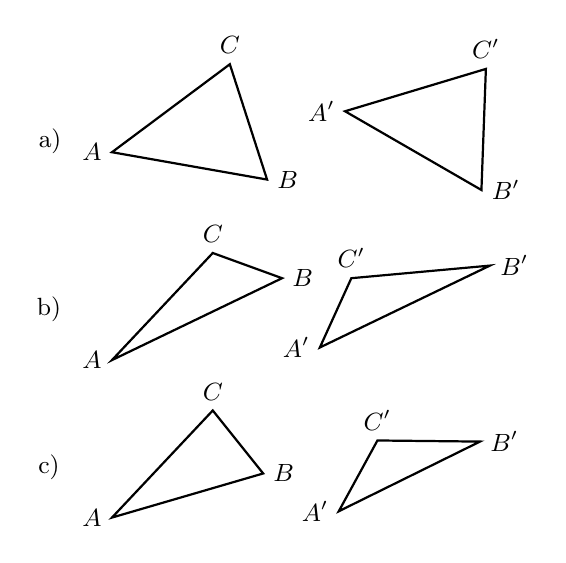
\begin{tikzpicture}[scale=0.8,font=\small]
\usetikzlibrary{calc}

\begin{scope}[rotate=-10]
\coordinate (a) at (0,0);
\coordinate (c) at (1.6,1.7);
\coordinate (b) at (2.5,0);
\draw[thick] (b) node[right] {$B$} -- (c) node[above] {$C$} -- (a) node[left] {$A$} -- cycle;
\node at (-1,0) {a)};
\end{scope}

\begin{scope}[xshift=3.7cm,yshift=0.65cm,rotate=-30]
\coordinate (a) at (0,0);
\coordinate (c) at (1.6,1.7);
\coordinate (b) at (2.5,0);
\draw[thick] (b) node[right] {$B'$} -- (c) node[above] {$C'$} -- (a) node[left] {$A'$} -- cycle;
\end{scope}

\begin{scope}[yshift=-3.3cm]
\coordinate (a) at (0,0);
\coordinate (c) at (1.6,1.7);
\coordinate (b) at (2.7,1.3);
\draw[thick] (b) node[right] {$B$} -- (c) node[above] {$C$} -- (a) node[left] {$A$} -- cycle;
\node at (-1,0.8) {b)};
\end{scope}

\begin{scope}[xshift=3.3cm,yshift=-3.1cm]
\coordinate (a) at (0,0);
\coordinate (c) at (0.5,1.1);
\coordinate (b) at (2.7,1.3);
\draw[thick] (b) node[right] {$B'$} -- (c) node[above] {$C'$} -- (a) node[left] {$A'$} -- cycle;
\end{scope}

\begin{scope}[yshift=-5.8cm]
\coordinate (a) at (0,0);
\coordinate (c) at (1.6,1.7);
\coordinate (b) at (2.4,0.7);
\draw[thick] (b) node[right] {$B$} -- (c) node[above] {$C$} -- (a) node[left] {$A$} -- cycle;
\node at (-1,0.8) {c)};
\end{scope}

\begin{scope}[xshift=3.6cm,yshift=-5.7cm,rotate=10]
\coordinate (a) at (0,0);
\coordinate (c) at (0.8,1);
\coordinate (b) at (2.4,0.7);
\draw[thick] (b) node[right] {$B'$} -- (c) node[above] {$C'$} -- (a) node[left] {$A'$} -- cycle;
\end{scope}


\end{tikzpicture}

\end{minipage}
\end{esercizio}

\begin{multicols}{2}

\subsubsection*{Dimostra le seguenti affermazioni, utilizzando il 
1\textsuperscript{o} e il 2\textsuperscript{o} criterio di congruenza 
dei triangoli.}

\begin{esercizio}
\label{ese:2.5}
In un triangolo \(ABC\) prolunga la mediana \(AM\) di un segmento \(MD\) 
congruente a \(MA\). Dimostra che il triangolo \(AMC\) è congruente al 
triangolo \(BMD\) e che il triangolo \(ABM\) è congruente al triangolo 
\(CMD\).
\end{esercizio}

\begin{esercizio}
\label{ese:2.6}
Due triangoli \(ABC\) e \(DEF\) hanno il lati \(AB\) e \(DE\) congruenti, 
hanno inoltre gli angoli esterni ai vertici \(A\) e \(B\) rispettivamente 
congruenti agli angoli esterni ai vertici \(D\) ed \(E\). Dimostra che i 
due triangoli sono congruenti.
\end{esercizio}

\begin{esercizio}
\label{ese:2.8}
Due triangoli rettangoli sono congruenti se hanno rispettivamente 
congruenti i due cateti.
\end{esercizio}

\begin{esercizio}
\label{ese:2.9}
Due triangoli rettangoli sono congruenti se hanno congruenti un 
cateto e l'angolo acuto adiacente ad esso.
\end{esercizio}

\begin{esercizio}
\label{ese:2.11}
Nel triangolo isoscele \(ABC\), di base \(BC\), prolunga la bisettrice 
\(AD\) di un segmento \(DE\). Dimostra che \(AE\) è bisettrice dell'angolo 
\(B\widehat{E}C\).
\end{esercizio}

\begin{esercizio}
\label{ese:2.13}
Siano \(ABC\) e \(DEF\) due triangoli congruenti. Sui lati congruenti 
\(AB\) e \(DE\) prendi il punto \(G\) su \(AB\) e \(H\) su \(DE\), in modo che 
\(AG\cong DH\). Dimostra che anche \(GC\) è congruente ad \(HF\).
\end{esercizio}

\begin{esercizio}
\label{ese:2.17}
Sui prolungamenti oltre \(A\) del lato \(AC\), oltre \(B\) del lato \(AB\) e 
oltre \(C\) del lato \(BC\) di un triangolo equilatero \(ABC\) si 
considerino i segmenti congruenti \(AA'\), \(BB'\), \(CC'\). Dimostrare che 
il triangolo \(A'B'C'\) è ancora equilatero.
\end{esercizio}

\begin{esercizio}
\label{ese:2.18}
Dato l'angolo convesso \(b\widehat{A}c\) si considerino su \(b\) i due 
punti \(B\) e \(B'\) e su \(c\) i punti \(C\) e \(C'\), tali che \(AB\) e \(AB'\) 
siano rispettivamente congruenti con \(AC\) e \(AC'\). Dimostrare che 
\(BB'\) e \(BC'\) sono rispettivamente congruenti con \(CC'\) e \(B'C\).
\end{esercizio}

\begin{esercizio}
\label{ese:2.19}
Dato un segmento \(AB\), condurre per il suo punto medio \(M\) una 
qualsiasi retta \(r\) e considerare su di essa, da parti opposte 
rispetto ad \(AB\), due segmenti congruenti \(MC\) e \(MD\). Dimostrare che 
i triangoli \(AMC\) e \(BMD\) sono congruenti.
\end{esercizio}

\begin{esercizio}
\label{ese:2.23}
Sui lati \(a\) e \(b\) di un angolo di vertice \(O\) prendi i punti \(A\) e 
\(B\) sulla semiretta \(a\) e i punti \(C\) e \(D\) sulla semiretta \(b\), in 
modo che \(OA\cong OC\) e \(AB\cong CD\). Sia \(E\) il punto di 
intersezione di \(AD\) con \(BC\). Dimostra che sono congruenti i 
triangoli \(ABE\) e \(CDE\).
\end{esercizio}

\begin{esercizio}
\label{ese:2.24}
Sia \(C\) un punto della bisettrice dell'angolo convesso 
\(a\widehat{O}b\), \(A\) un punto sul lato \(a\) e \(B\) un punto sul lato 
\(b\), tali che \(OA\cong OB\). Dimostra che i triangoli \(BCO\) e \(ACO\) 
sono congruenti.
\end{esercizio}

\subsubsection*{Dimostra le seguenti affermazioni sui triangoli 
isosceli.}

\begin{esercizio}
\label{ese:2.28}
In un triangolo isoscele le mediane relative ai lati congruenti sono 
congruenti. 
\end{esercizio}

\begin{esercizio}
\label{ese:2.29}
In un triangolo isoscele le bisettrici degli angoli alla base sono 
congruenti. 
\end{esercizio}

\begin{esercizio}
\label{ese:2.30}
Due triangoli isosceli sono congruenti se hanno rispettivamente 
congruenti l'angolo al vertice e uno dei lati obliqui.
\end{esercizio}

\begin{esercizio}
\label{ese:2.31}
Due triangoli isosceli sono congruenti se hanno rispettivamente 
congruenti la base e uno degli angoli ad essa adiacenti.
\end{esercizio}

\begin{esercizio}
\label{ese:2.32}
Due triangoli isosceli sono congruenti se hanno rispettivamente 
congruenti la base e la bisettrice dell'angolo al vertice.
\end{esercizio}

\begin{esercizio}
\label{ese:2.34}
Sia \(P\) il punto di intersezione delle bisettrici degli angoli alla 
base \(AB\) di un triangolo isoscele \(ABC\). Dimostra che anche \(APB\) è 
isoscele.
\end{esercizio}

\begin{esercizio}
\label{ese:2.36}
In un triangolo isoscele \(ABC\) di base \(AB\) e vertice \(C\), indica con 
\(M\) il punto medio di \(AC\), con \(N\) il punto medio di \(CB\) e con \(H\) 
il punto medio di \(AB\). Quali delle seguenti coppie di triangoli sono 
congruenti? Dimostralo.
\begin{multicols}{2}
\begin{enumeratea}
\item \(AMH\) e \(HNB\)
\item \(MNH\) e \(MNC\)
\item \(AMH\) e \(MCN\)
\end{enumeratea}
\end{multicols}
\end{esercizio}

\begin{esercizio}
\label{ese:2.38}
In un triangolo isoscele \(ABC\) di base \(AB\) e vertice \(C\) prolunga la 
base \(AB\), dalla parte di \(A\) di un segmento \(AD\) e dalla parte di 
\(B\) di un segmento \(BE\) congruente ad \(AD\). Dimostra che anche il 
triangolo \(DEC\) è isoscele.
\end{esercizio}

\begin{esercizio}
\label{ese:2.40}
Due triangoli isosceli \(ABC\) e \(ABD\) hanno in comune la base \(AB\), i 
vertici \(C\) e \(D\) sono situati da parti opposte rispetto alla base 
\(AB\). Dimostra che la retta per \(CD\) è bisettrice dell'angolo in \(C\).
\end{esercizio}

\begin{esercizio}
\label{ese:2.45}
In un triangolo isoscele \(ABC\) di base \(AB\) e vertice \(C\), prendi su 
\(AC\) un punto \(D\) e su \(CB\) un punto \(E\) in modo che \(CD\cong CE\). 
Dimostra che il triangolo \(DME\), dove \(M\) è il punto medio della base 
\(AB\), è isoscele.
\end{esercizio}

\begin{esercizio}
\label{ese:2.46}
Due triangoli isoscele hanno in comune la base, dimostra che la retta 
che unisce i vertici dei due triangoli divide la base a metà.
\end{esercizio}

\begin{esercizio}
\label{ese:2.49}
Si prolunghino i lati \(AC\) e \(CB\) del triangolo isoscele \(ABC\) 
rispettivamente di due segmenti \(CP\) e \(CQ\) tra loro congruenti. 
Dimostrare che \(A\widehat{Q}B\cong A\widehat{P}Q\) e che 
\(A\widehat{B}P\cong Q\widehat{A}B\).
\end{esercizio}

\subsubsection*{Esercizi sui criteri di congruenza dei triangoli e 
sui triangoli isosceli.}

\begin{esercizio}
\label{ese:2.54}
Due triangoli sono congruenti se hanno
\begin{enumeratea}
\item tre lati congruenti \hfill\boxV\quad\boxF
\item tre angoli congruenti \hfill\boxV\quad\boxF
\item due lati e l'angolo compreso congruenti\tab\hfill\boxV\quad\boxF
\item due angoli e il lato in comune 
congruenti\tab\hfill\boxV\quad\boxF
\item un lato e l'angolo opposto 
congruenti\tab\tab\hfill\boxV\quad\boxF
\end{enumeratea}
\hfill[a)~V,\quad b)~F,\quad c)~V,\quad d)~V,\quad e)~F]
\end{esercizio}

\begin{esercizio}
\label{ese:2.58}
Se in due triangoli sono congruenti due coppie di lati e la mediana 
relativa ad uno di essi, allora i due triangoli sono congruenti.
\end{esercizio}

\begin{esercizio}
\label{ese:2.59}
Se in due triangoli sono congruenti due coppie di lati e la 
bisettrice relativa ad uno di essi, allora i due triangoli sono 
congruenti.
\end{esercizio}

\begin{esercizio}
\label{ese:2.63}
In un triangolo isoscele \(ABC\) di base \(BC\) e vertice \(A\) prendi un 
punto \(D\) sul lato \(AB\) e un punto \(E\) sul lato \(AC\), in modo che 
\(BD\cong EC\), unisci \(C\) con \(D\) e \(B\) con \(E\). Sia \(F=BE\cap DC\). 
Dimostra che i triangoli \(BFA\) e \(CFA\) sono congruenti.
\end{esercizio}

\begin{esercizio}
\label{ese:2.65}
In un triangolo isoscele \(ABC\) di base \(BC\) e vertice \(A\), prolunga 
il lato \(AB\) di un segmento \(BD\) e il lato \(AC\) di un segmento \(CE\) 
in modo che \(BD\cong CE\), prolunga la base \(BC\) di un segmento \(BG\), 
dalla parte di \(B\), e di un segmento \(CF\) dalla parte di \(C\), in modo 
che \(BG\cong CF\). Dimostra che sono congruenti i triangoli \(ADG\) e 
\(AEF\).
\end{esercizio}

\begin{esercizio}
\label{ese:2.66}
In un triangolo scaleno \(ABC\) sia \(AC>BC\). Prolunga \(BC\), dalla parte 
di \(C\), di un segmento \(CD\) congruente ad \(AC\) e prolunga \(AC\), dalla 
parte di \(C\), di un segmento \(CE\) congruente a \(BC\). Detto \(H\) il 
punto di intersezione della retta per \(AB\) con la retta per \(DE\), 
dimostra che \(AH\cong DH\).
\end{esercizio}

\begin{esercizio}
\label{ese:2.67}
In un triangolo isoscele \(ABC\) di base \(BC\) e vertice \(A\), prolunga 
il lato \(AB\) di un segmento \(BD\) e il lato \(AC\) di un segmento \(CE\) 
in modo che \(BD\cong CE\). Unisci \(D\) con \(C\) e prolunga il segmento 
\(DC\), dalla parte di \(C\) di un segmento \(CF\). Unisci \(E\) con \(B\) e 
prolunga il segmento \(EB\) dalla parte di \(B\) di un segmento \(BG\cong 
CF\). Dimostra che i triangoli \(AGD\) e \(AFE\) sono congruenti.
\end{esercizio}

\begin{esercizio}
\label{ese:2.68}
Dato il triangolo convesso non piatto \(a\widehat{O}b\) si prenda un 
punto \(A\) sul lato \(Oa\) e un punto \(B\) sul lato \(Ob\), in modo che 
\(OA\cong OB\). Sia \(M\) il punto medio di \(OA\) e \(N\) il punto medio di 
\(OB\), congiungi \(A\) con \(N\) e \(B\) con \(M\), indica con \(P\) in punto di 
intersezione. Dimostra che sono congruenti i triangoli \(OBC\) e \(OAD\) 
e i triangoli \(AOP\) e \(OPB\).
\end{esercizio}

\begin{esercizio}
\label{ese:2.71}
Sia \(P\) un punto interno al triangolo isoscele \(ABC\) di base \(AB\) e 
sia \(AP\cong PB\). Si dimostri che \(CP\) appartiene alla bisettrice 
dell'angolo in \(C\).
\end{esercizio}

\begin{esercizio}
\label{ese:2.81}
Sia \(P\) un punto interno al triangolo isoscele \(ABC\), di base \(AB\). 
Dimostra che se \(P\widehat{A}C\cong P\widehat{C}B\) allora \(P\) si 
trova sulla bisettrice dell'angolo in \(A\).
\end{esercizio}

\begin{esercizio}
\label{ese:2.89}
Sulla bisettrice \(c\) di un angolo \(a\widehat{O}b\) prendi un punto \(P\) 
e traccia da esso le perpendicolari ai lati \(a\) e \(b\) dell'angolo che 
incontrano rispettivamente in \(A\) e in \(B\) i suddetti lati. Dimostra 
che \(OA\cong OB\).
\end{esercizio}

\end{multicols}

\begin{esercizio}[Prove invalsi 2006]
\label{ese:2.99}
Osserva la figura a lato. Se \(AB\not\cong AC\) e \(BH\cong HC\), che 
cosa rappresenta il segmento \(AH\) nel triangolo \(ABC\)?\\
\begin{minipage}{.5\linewidth}
\begin{enumeratea}
\item Un'altezza.
\item Una mediana.
\item Una bisettrice.
\item Un asse.
\end{enumeratea}
\end{minipage}\hfil
\begin{minipage}{.2\linewidth}
  \centering
    % Copyright (c) 2015 Daniele Masini - d.masini.it@gmail.com

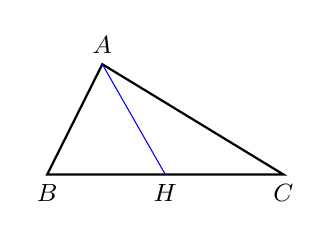
\begin{tikzpicture}[scale=1,font=\small]
\usetikzlibrary{calc}

\begin{scope}

\coordinate (b) at (0,0);
\coordinate (a) at (0.7,1.4);
\coordinate (c) at (3,0);

\draw[thick] (b) node[below] {$B$} -- (c) node[below] {$C$} -- (a) node[above] {$A$} -- cycle;

\coordinate (h) at ($(b)!0.5!(c)$);

\draw[blue] (h) node[black,below] {$H$} -- (a); % mediana
\end{scope}

\end{tikzpicture}

\end{minipage}
\hfill[b]
\end{esercizio}

\begin{esercizio}[Prove invalsi 2003]
\label{ese:2.100}
Da un triangolo equilatero \(MNO\) di lato 6~cm viene tagliato via un 
triangolo equilatero di vertice in \(O\) e lato 2~cm. Il perimetro del 
quadrilatero rimanente è \ldots
\begin{multicols}{5}
\begin{enumeratea}
\item 12~cm;
\item 14~cm;
\item 16~cm;
\item 18~cm;
\item 20~cm.
\end{enumeratea}
\end{multicols}
\hfill[c]
\end{esercizio}
